\setcounter{section}{5}
\setlength{\parindent}{0pt}
\setlength{\parskip}{6pt}

\section{Design Front-end}
In questo capitolo vengono presentati i mockup e le schermate definitive dell'applicazione Rinova. Le interfacce sono state progettate per garantire la massima usabilità (RNF-08) e responsività (RNF-11), soddisfacendo puntualmente tutti i requisiti funzionali descritti nei capitoli precedenti.

\subsection{Onboarding e Accesso}
Questa sezione descrive le interfacce dedicate all'identificazione e alla registrazione degli utenti, punto di ingresso per tutte le tipologie di attori (Utenti, Admin CER, Staff).

\subsubsection*{Registrazione Utente}
\begin{figure}[H]
    \centering
    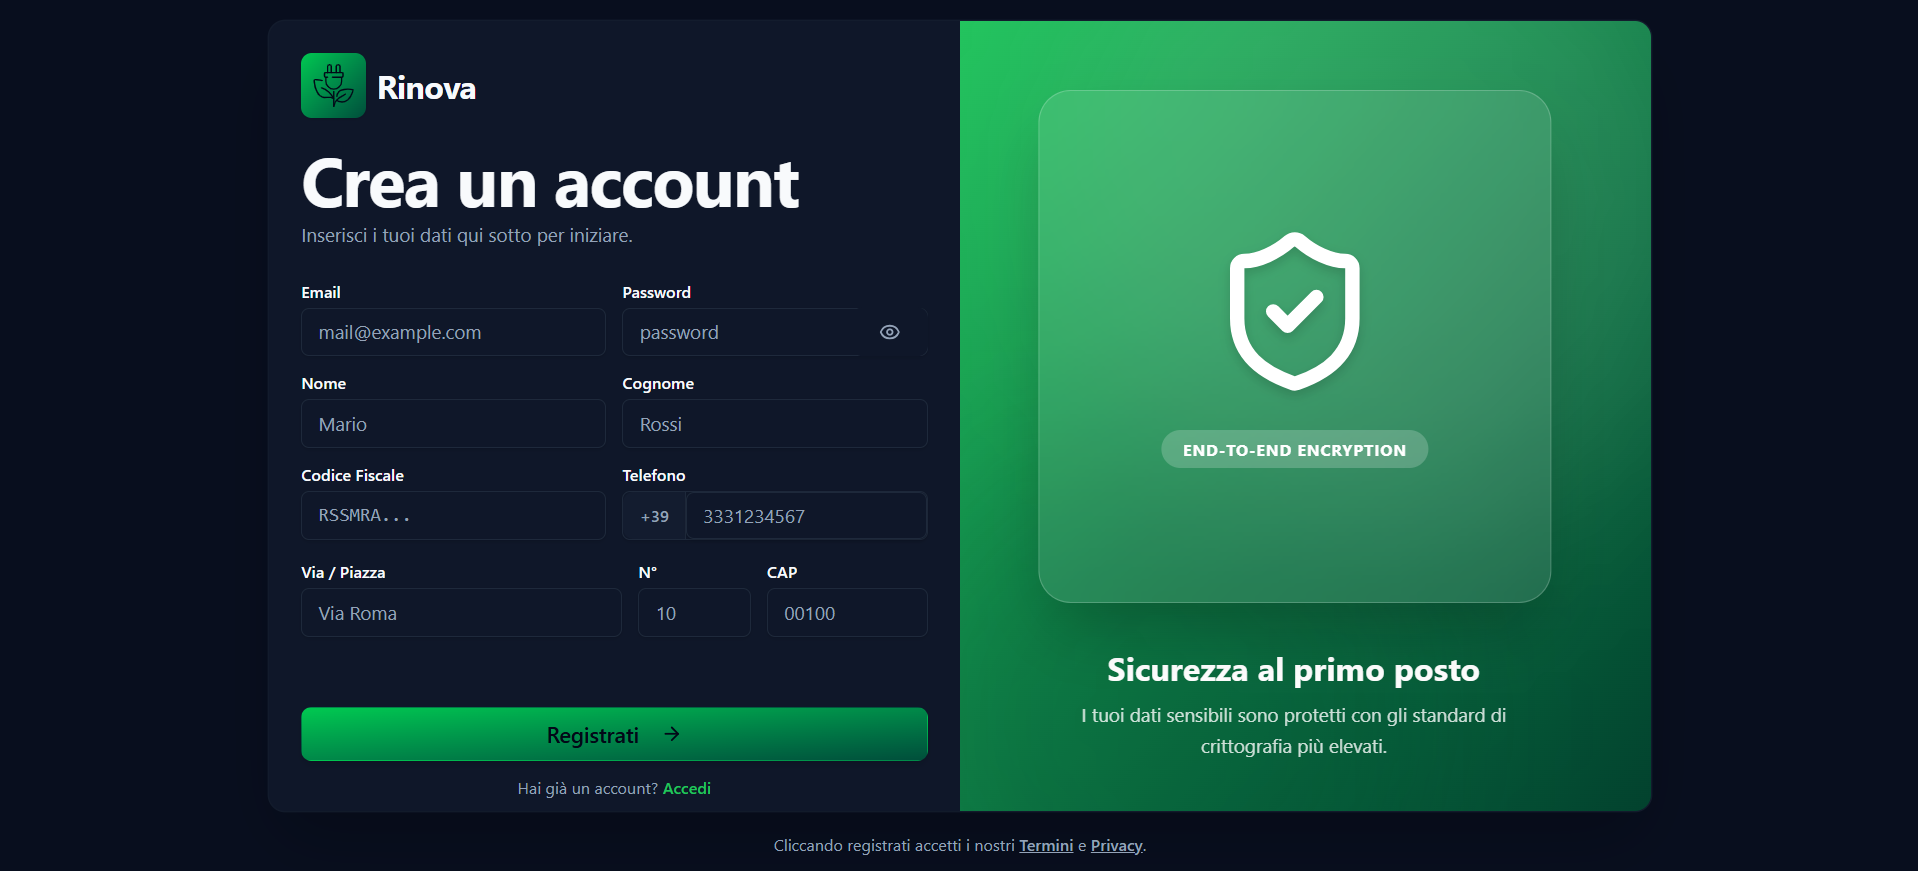
\includegraphics[width=1\textwidth]{images/frontend/schermata_registrazione.png}
    \caption{Schermata di Registrazione}
    \label{fig:registrazione}
\end{figure}

La Figura \ref{fig:registrazione} mostra il modulo di iscrizione alla piattaforma.

\textbf{RF-01 - Registrazione utente:}
L'interfaccia richiede l'inserimento di tutti i dati anagrafici obbligatori. Il sistema effettua una validazione in tempo reale dei campi e, tramite il pulsante "Registrati", finalizza la creazione del profilo inviando una mail di conferma.

\textbf{Navigazione:}
Il link "Hai già un account? Accedi" permette il passaggio rapido alla schermata di login, separando chiaramente i flussi operativi.

\subsubsection*{Autenticazione}
\begin{figure}[H]
    \centering
    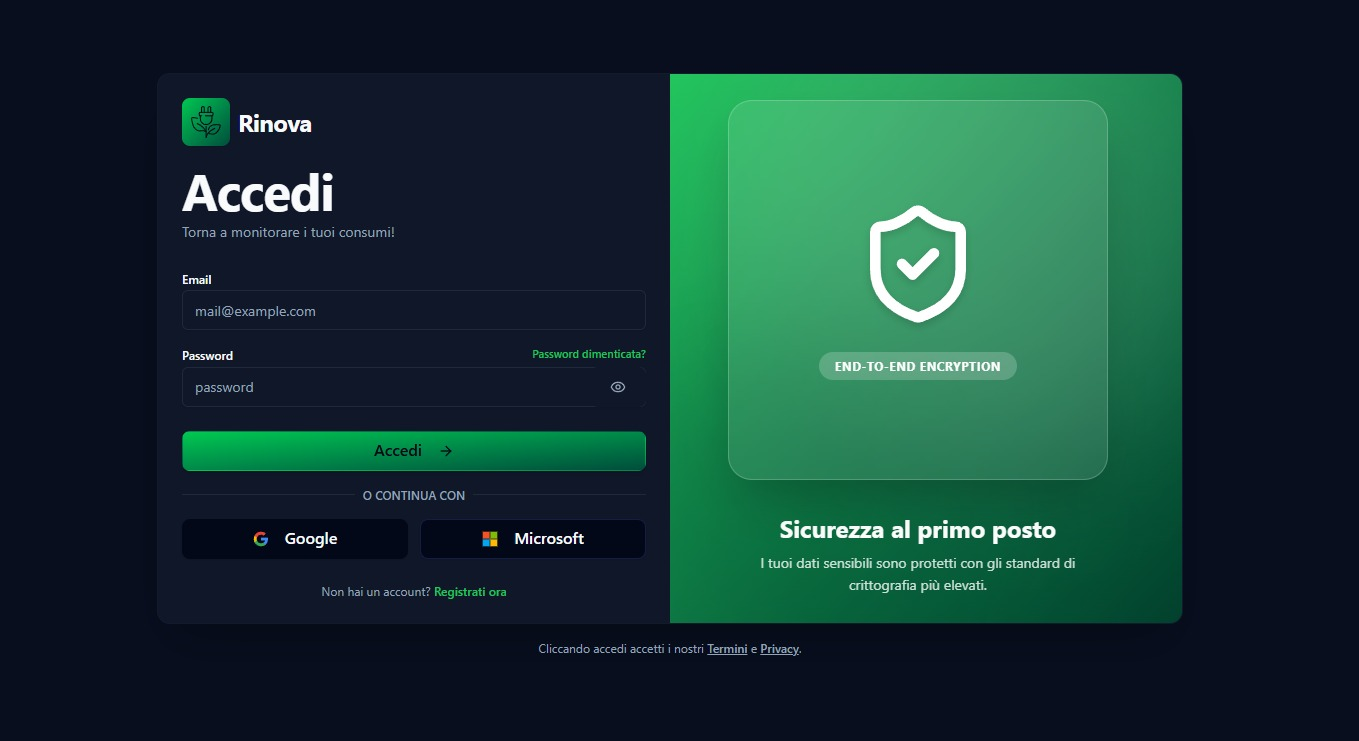
\includegraphics[width=1\textwidth]{images/frontend/schermata_login.jpeg}
    \caption{Schermata di Accesso}
    \label{fig:accesso}
\end{figure}

La Figura \ref{fig:accesso} illustra l'interfaccia di login unificata.

\textbf{RF-02 - Login utente:}
Il modulo centrale permette l'accesso tramite credenziali (email/password), fornendo feedback visivi immediati in caso di errore (RNF-12).

\textbf{Integrazione OAuth:}
I pulsanti per l'autenticazione tramite Google e Microsoft soddisfano il requisito di accesso rapido tramite provider esterni.

\textbf{RF-02.1 - Recupero Password:}
Il collegamento "Password dimenticata?" avvia il flusso di ripristino delle credenziali via email.

\textbf{RNF-05 - Sicurezza:}
Tutti i dati di autenticazione sono trasmessi su protocollo crittografato HTTPS. L'integrazione con provider OAuth (Google/Microsoft) delega la gestione delle credenziali a sistemi sicuri certificati, riducendo la superficie di attacco.

\newpage

\subsection{Monitoraggio Energetico}
Il "cuore" dell'applicazione, dove l'utente visualizza i dati energetici personali (RF-05) e scarica la reportistica (RF-06).

\subsubsection*{Dashboard e Panoramica Energetica}
\begin{figure}[H]
    \centering
    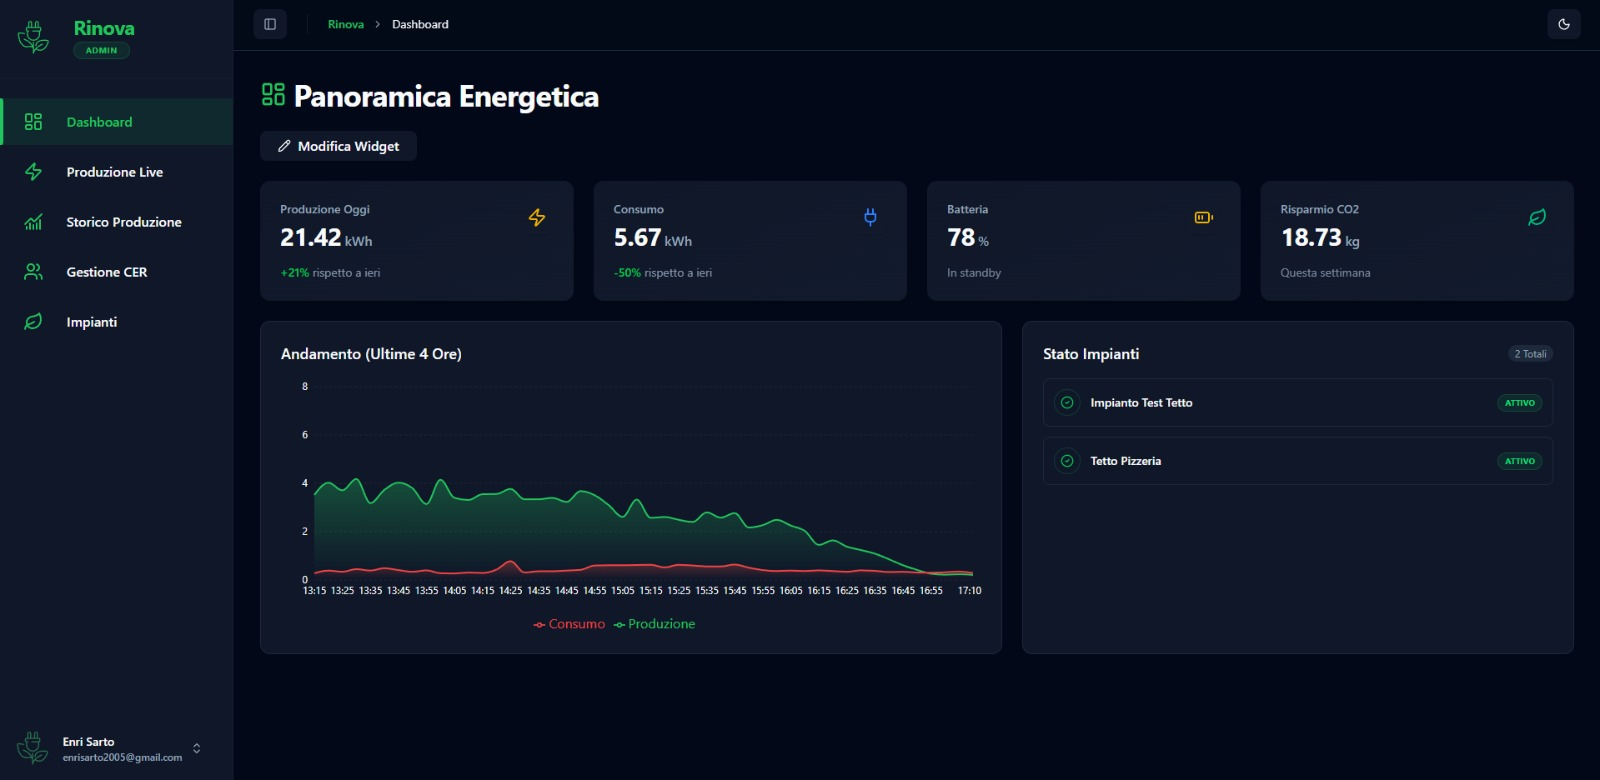
\includegraphics[width=1\textwidth]{images/frontend/schermata_dashboard.png}
    \caption{Dashboard Principale - Panoramica Energetica}
    \label{fig:dashboard_panoramica}
\end{figure}

La Figura \ref{fig:dashboard_panoramica} illustra la Dashboard principale dell'applicazione, concepita come centro di controllo unificato per l'utente.

\textbf{RF-05 - Visualizzazione dati energetici personali:}
La schermata soddisfa il requisito fornendo una visione d'insieme immediata tramite quattro widget principali (KPI) che mostrano i dati aggregati giornalieri:
\begin{itemize}
    \item \textbf{Produzione Oggi:} Il totale dell'energia generata dagli impianti rinnovabili.
    \item \textbf{Consumo:} Il prelievo energetico dell'utenza domestica.
    \item \textbf{Batteria:} La percentuale di carica attuale dei sistemi di accumulo.
    \item \textbf{Risparmio CO\textsubscript{2}:} L'impatto ambientale positivo generato nella settimana corrente.
\end{itemize}

\textbf{Analisi Temporale e Stato:}
Nella parte inferiore, il grafico "Andamento (Ultime 4 Ore)" offre un feedback visivo immediato sui trend di produzione e consumo a breve termine. A destra, il riquadro "Stato Impianti" notifica all'utente eventuali anomalie o disconnessioni degli impianti, garantendo una supervisione proattiva del sistema.

\textbf{RNF-08 - Usabilità e Personalizzazione:}
Il layout a griglia e l'uso di contrasti elevati (Dark Mode) facilitano la lettura rapida dei dati critici. La presenza di funzionalità per la modifica dei widget permette all'utente di adattare l'interfaccia alle proprie priorità.

\subsubsection*{Produzione Live}
\begin{figure}[H]
    \centering
    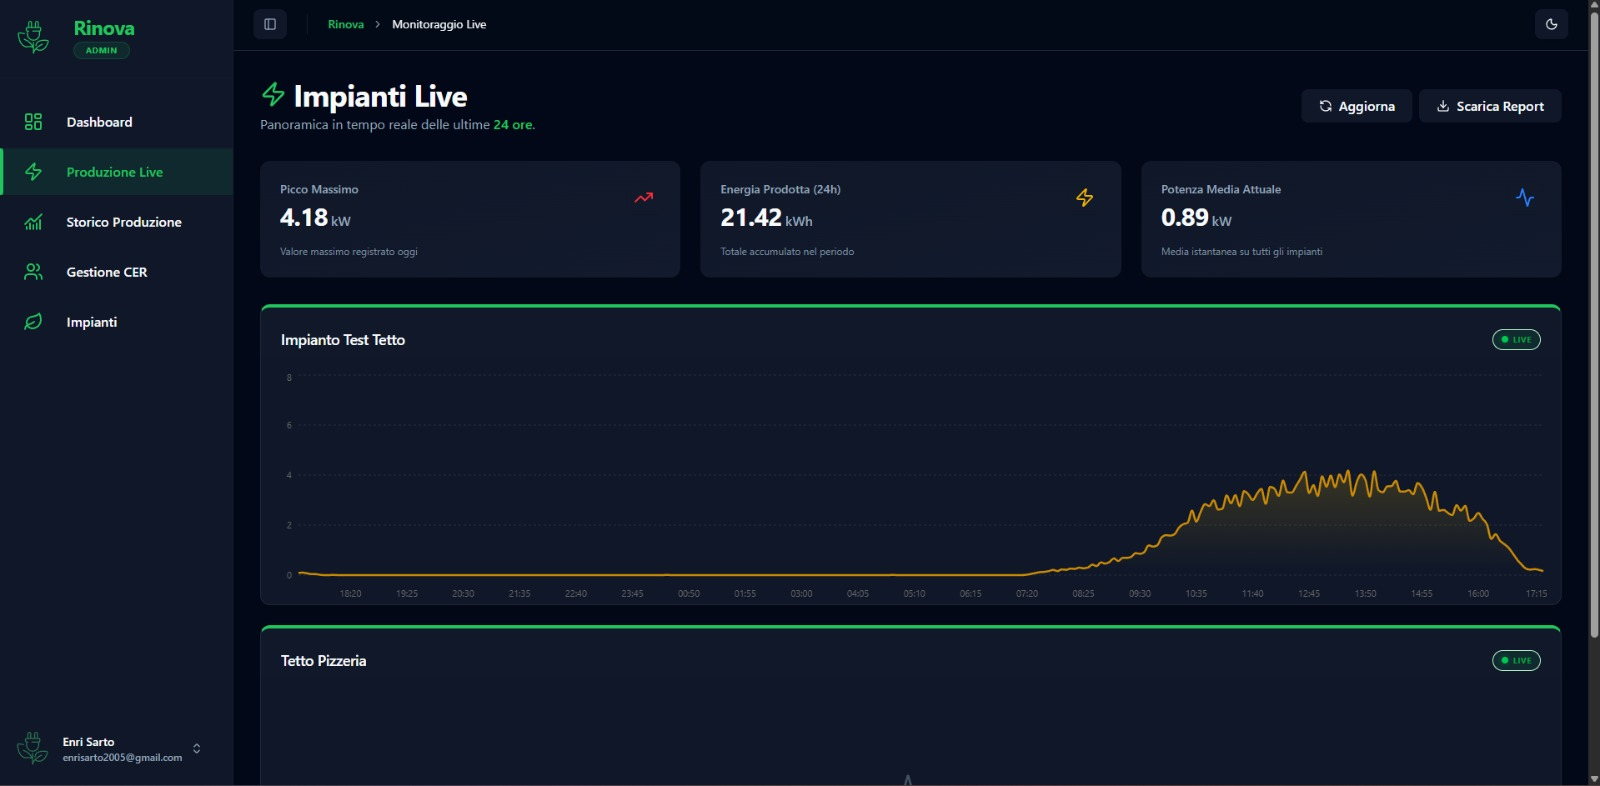
\includegraphics[width=1\textwidth]{images/frontend/schermata_live.png}
    \caption{Monitoraggio Produzione in Tempo Reale}
    \label{fig:produzione_live}
\end{figure}

La Figura \ref{fig:produzione_live} mostra i dati in tempo reale degli impianti.

\textbf{RF-05 - Visualizzazione dati energetici:}
Le card superiori mostrano i KPI istantanei: Picco Massimo, Energia Prodotta nelle 24h e Potenza Media Attuale. Lo stato operativo dell'impianto è indicato visivamente (badge verde "LIVE"), garantendo all'utente una comprensione immediata del funzionamento del sistema.

\textbf{RF-06 - Reportistica:}
In alto a destra è presente il pulsante "Scarica Report", che permette l'esportazione immediata dei dati visualizzati in formato PDF.

\subsubsection*{Storico e Analisi}
\begin{figure}[H]
    \centering
    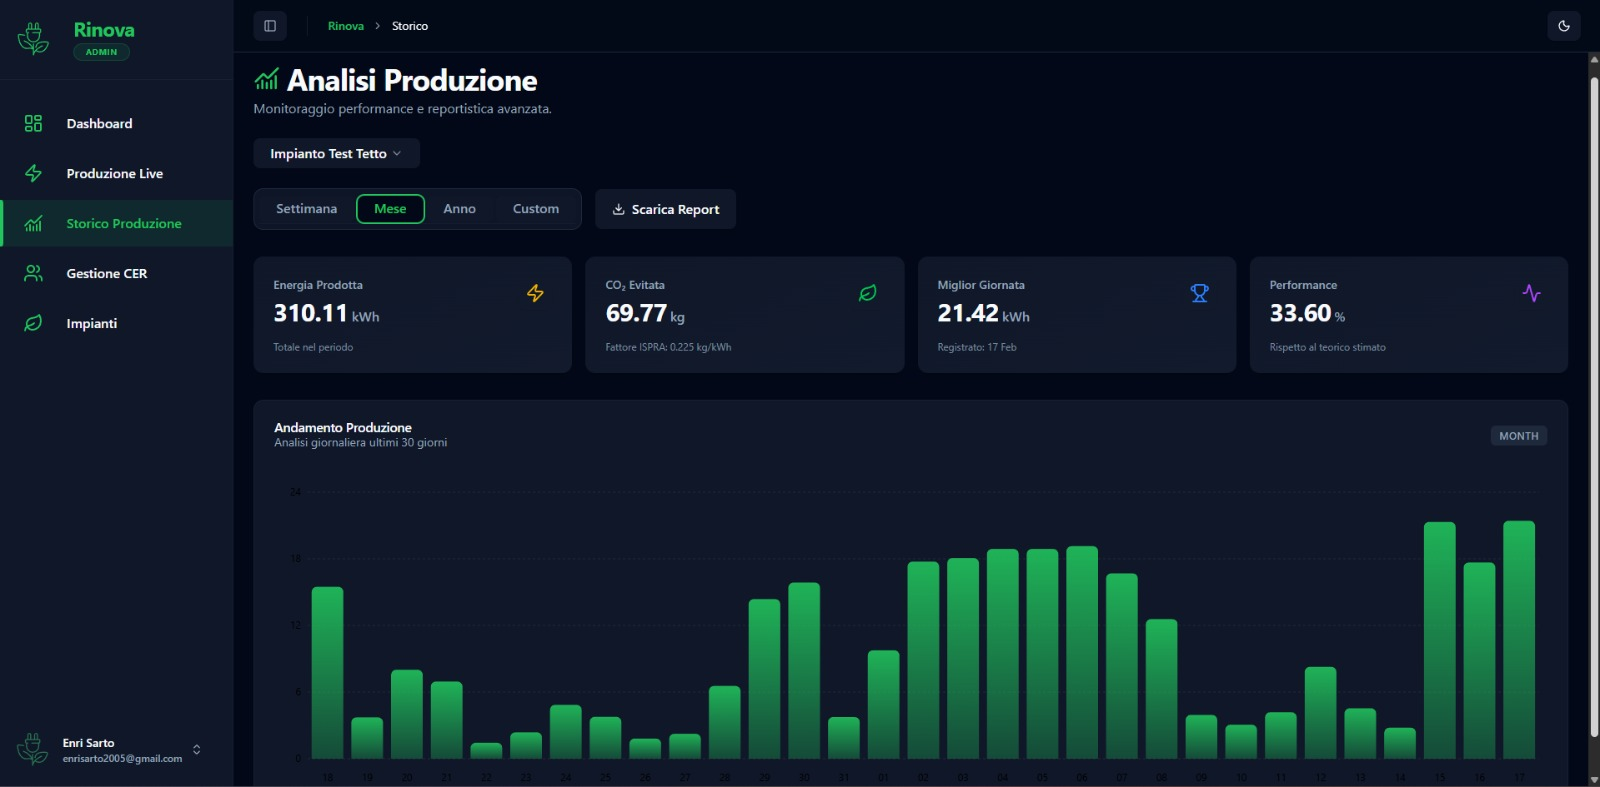
\includegraphics[width=1\textwidth]{images/frontend/schermata_storico.png}
    \caption{Analisi Storica della Produzione}
    \label{fig:storico_produzione}
\end{figure}

La Figura \ref{fig:storico_produzione} rappresenta la sezione di analisi approfondita.

\textbf{RF-05 - Visualizzazione dati (Storico):}
L'utente può filtrare i dati per intervalli temporali (Settimana, Mese, Anno, Custom) tramite i selettori dedicati. I widget mostrano metriche aggregate come la CO\textsubscript{2} evitata e la performance rispetto al teorico stimato.

\newpage

\subsection{Gestione Impianti}
Sezione dedicata alla configurazione tecnica degli asset di produzione (RF-07).

\subsubsection*{Lista e Dettaglio Impianti}
\begin{figure}[H]
    \centering
    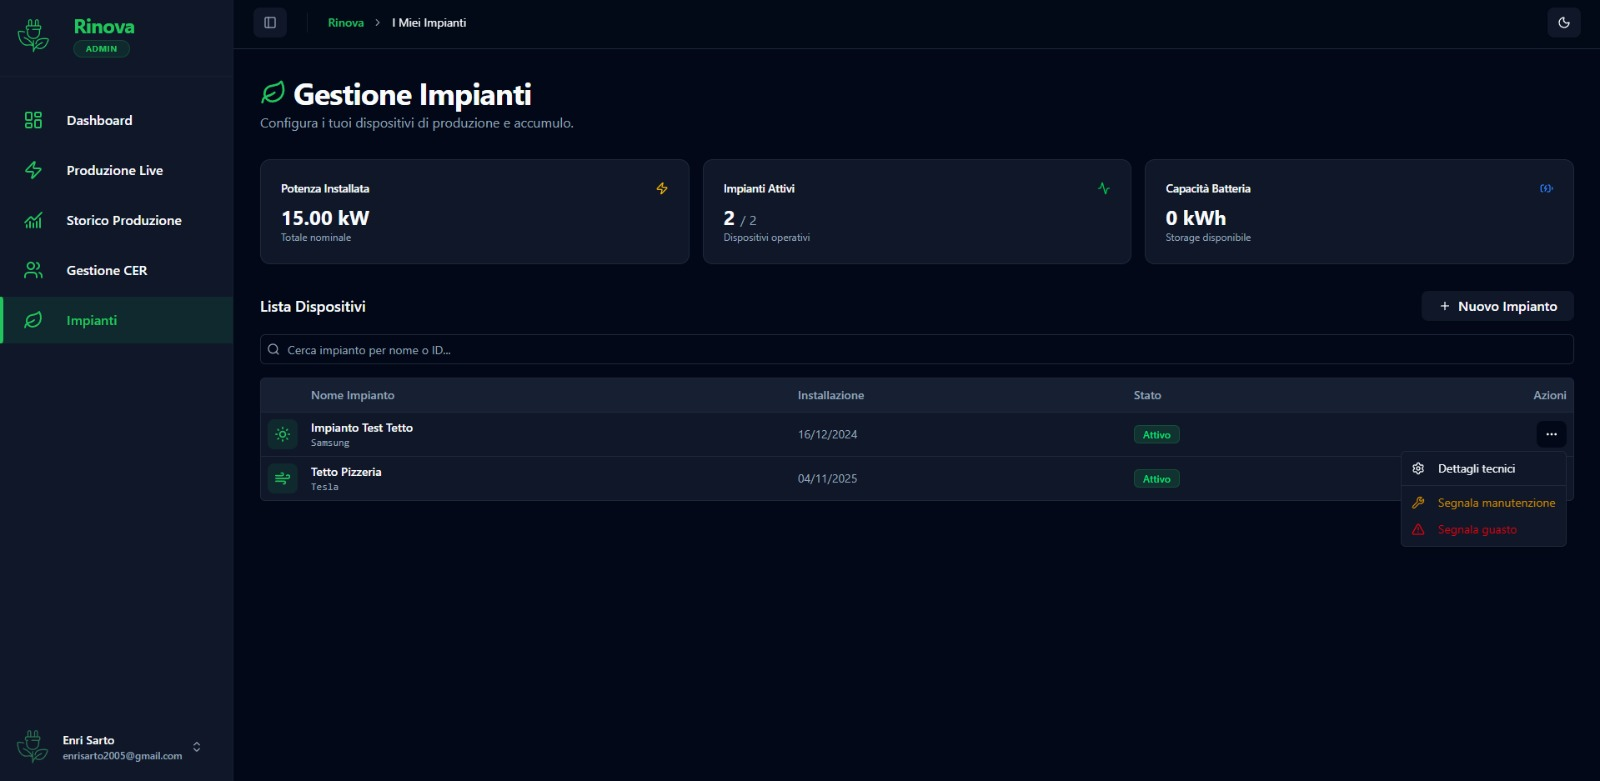
\includegraphics[width=1\textwidth]{images/frontend/schermata_impianti.png}
    \caption{Lista Impianti}
    \label{fig:impianti}
\end{figure}

\begin{figure}[H]
    \centering
    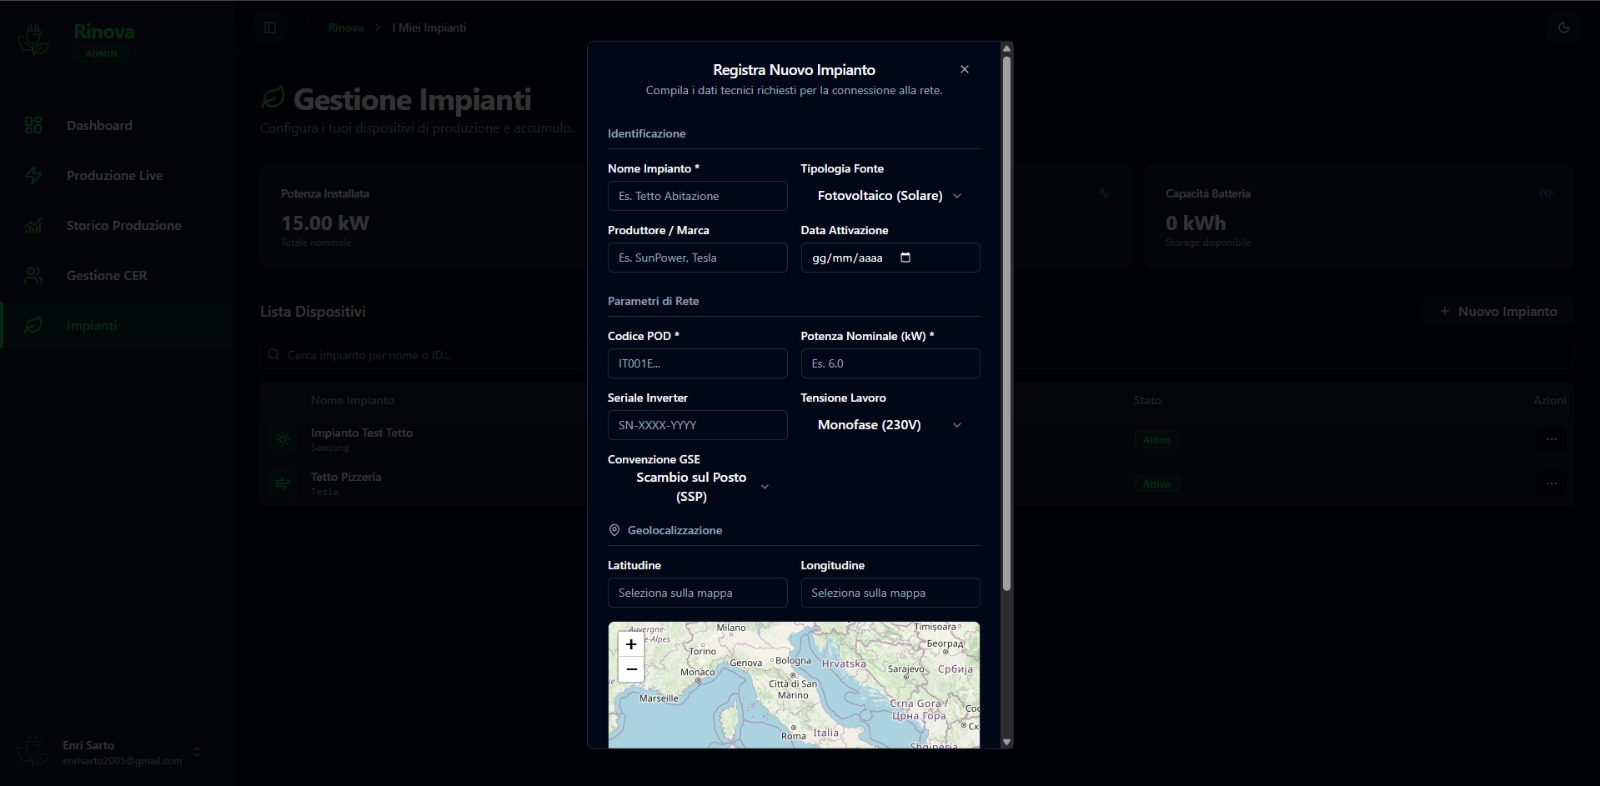
\includegraphics[width=1\textwidth]{images/frontend/schermata_impianti2.png}
    \caption{Aggiunta Impianto}
    \label{fig:impianti2}
\end{figure}

\begin{figure}[H]
    \centering
    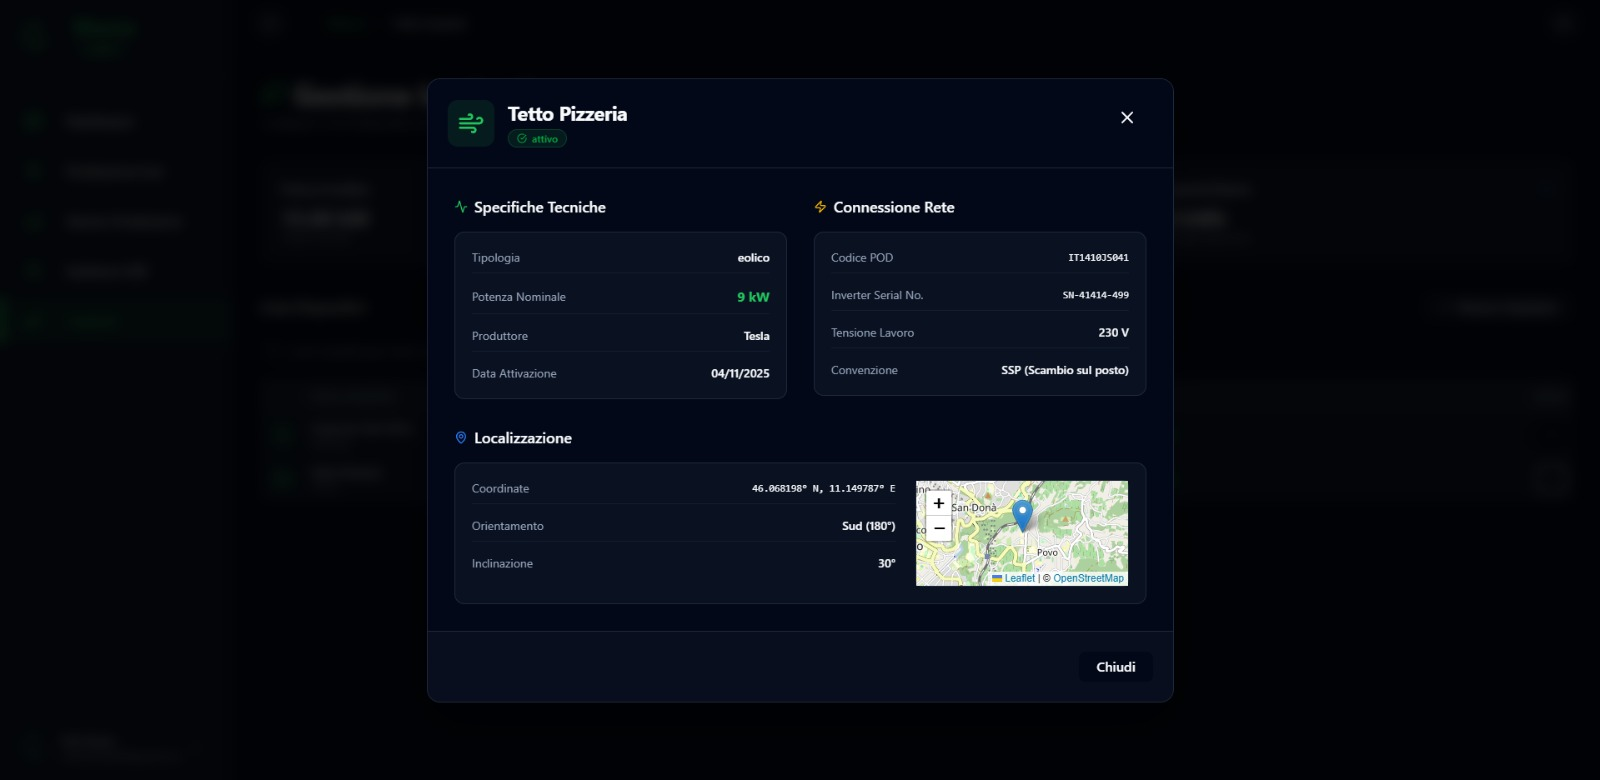
\includegraphics[width=1\textwidth]{images/frontend/schermata_impostazioni3.png.jpeg}
    \caption{Dettagli Impianto}
    \label{fig:impianti3}
\end{figure}

Le Figure \ref{fig:impianti}, \ref{fig:impianti2} e \ref{fig:impianti3} mostrano la pagina di gestione degli impianti.

\textbf{RF-07 - Gestione impianti energetici:}
La tabella riepilogativa permette di monitorare lo stato di tutti gli impianti registrati. Tramite il pulsante di aggiunta è possibile registrare nuovi asset inserendo codice identificativo, potenza e posizione, premendo invece "Dettagli tecnici" è possibile vedere i dettagli tecnici dell'impianto.

\newpage

\subsection{Ecosistema Comunità Energetiche (CER)}
Questa sezione copre sia l'interazione dell'utente semplice (Ricerca/Adesione) sia le funzionalità avanzate per gli Amministratori di CER.

\subsubsection*{Ricerca CER (Lato Utente)}
\begin{figure}[H]
    \centering
    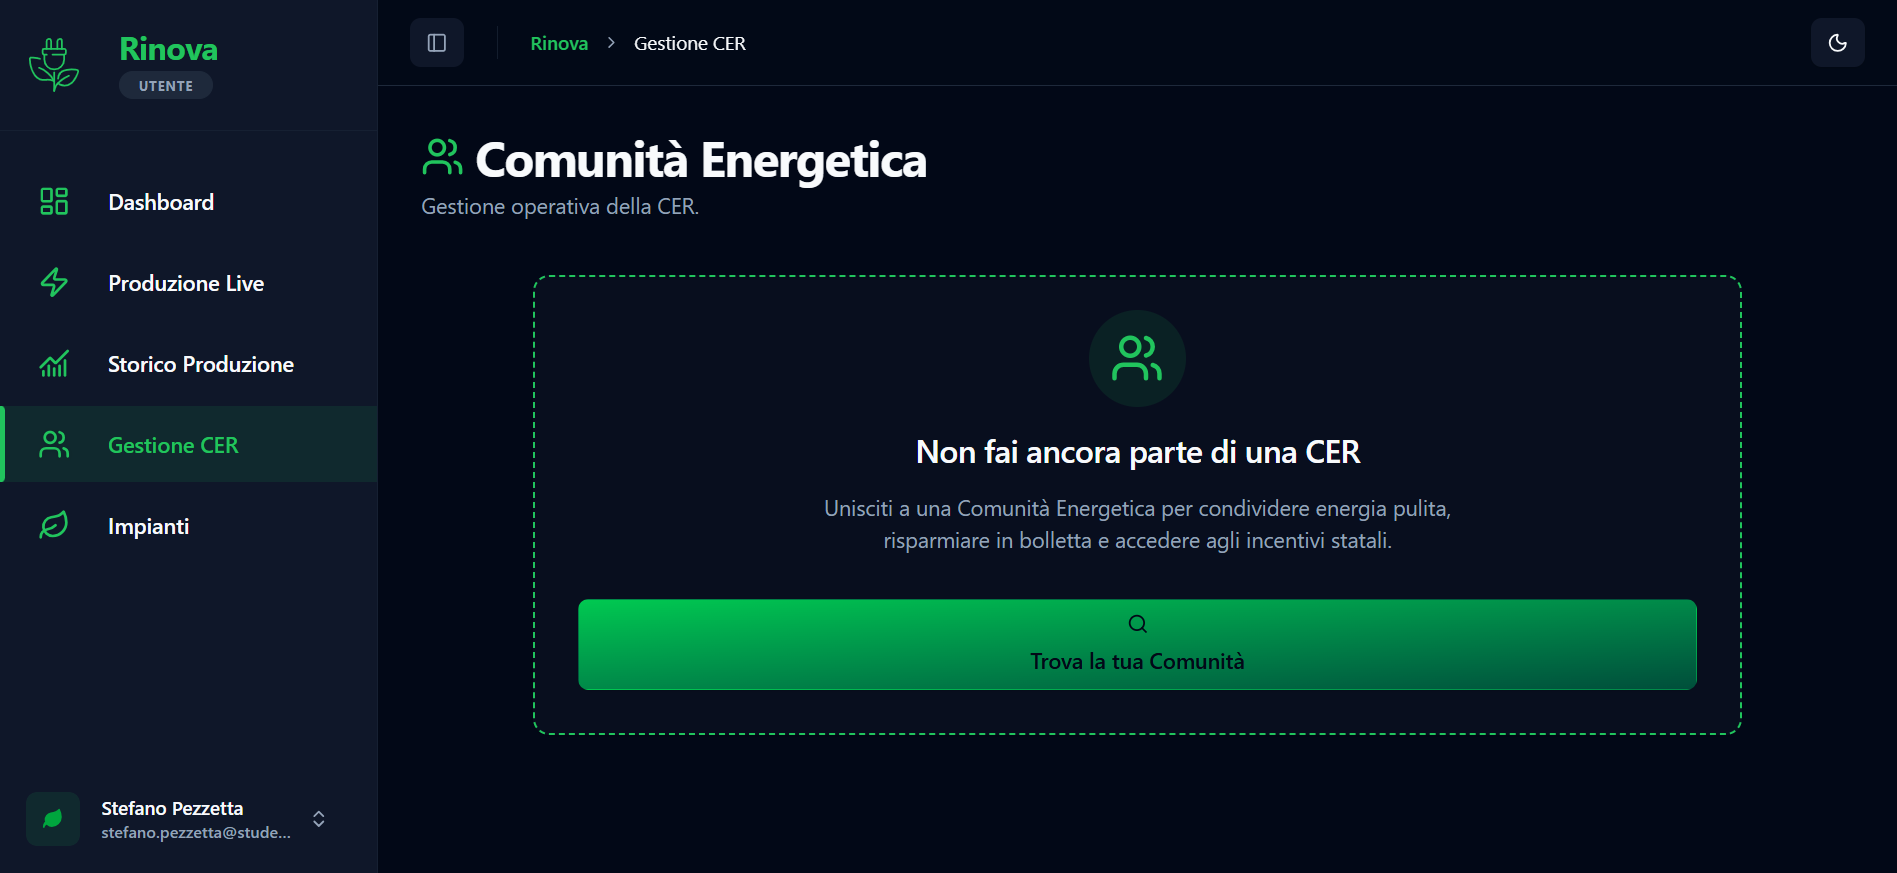
\includegraphics[width=1\textwidth]{images/frontend/schermata_cercaCer.png}
    \caption{Ricerca e Adesione CER}
    \label{fig:cercaCer}
\end{figure}

La Figura \ref{fig:cercaCer} mostra l'interfaccia per gli utenti non ancora associati.

\textbf{RF-08 e RF-09 - Ricerca e Adesione:}
La barra di ricerca permette di individuare una CER tramite nome o codice. Una volta trovata, l'utente può inviare una richiesta di adesione che rimarrà in attesa di approvazione.

\subsubsection*{Gestione CER (Lato Admin)}
\begin{figure}[H]
    \centering
    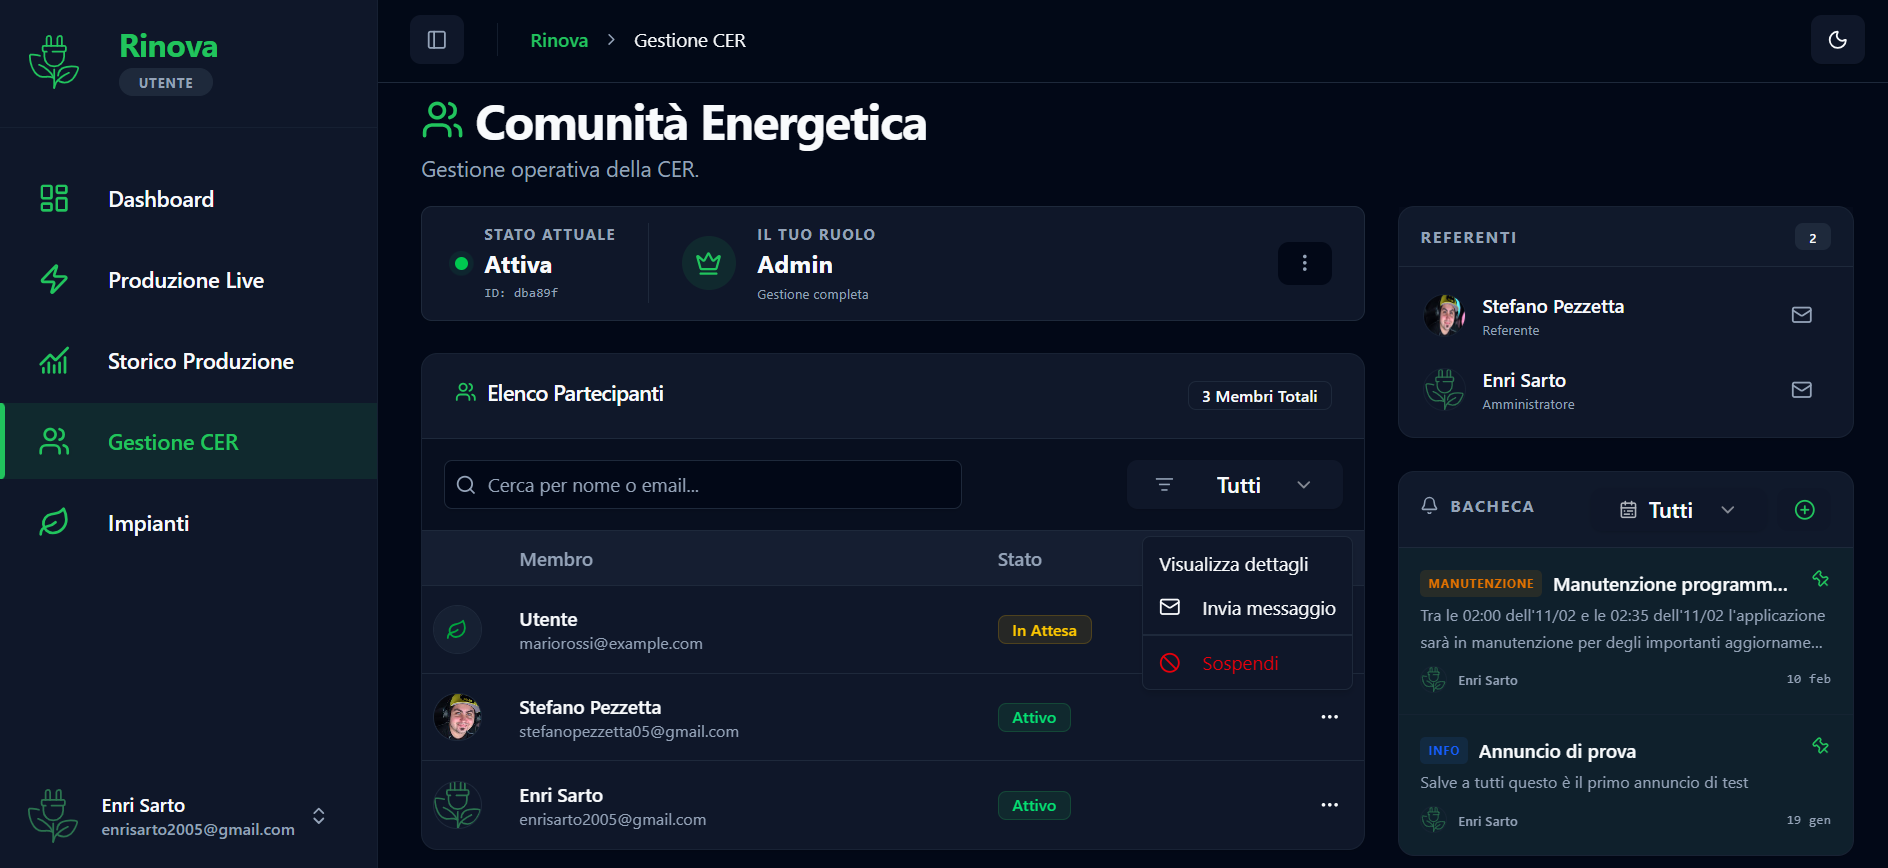
\includegraphics[width=1\textwidth]{images/frontend/schermata_cerAdmin.png}
    \caption{Dashboard di Gestione CER}
    \label{fig:gestione_cer}
\end{figure}

La Figura \ref{fig:gestione_cer} illustra il pannello di controllo riservato agli amministratori della comunità.

\textbf{RF-11 - Gestione Membri:}
La tabella "Elenco Partecipanti" mostra tutti gli utenti iscritti, permettendo di visualizzarne i dettagli e lo stato (es. "Attivo").

\textbf{RF-12 - Gestione Richieste:}
Come visibile nella figura, gli utenti che hanno fatto richiesta appaiono in lista con stato "In Attesa" (badge giallo). L'amministratore può modificarne lo stato attraverso il menù azioni.

\textbf{RF-14 - Gestione Bacheca:}
Sulla destra è presente il widget "Bacheca", dove l'amministratore può pubblicare avvisi (come l'avviso di "Manutenzione programmata" visibile in figura) per tutti i membri (RF-16 Notifiche).

\textbf{RNF-02 - Performance e Scalabilità:}
La tabella dei partecipanti è progettata per gestire un elevato numero di utenti utilizzando la paginazione e il caricamento asincrono, garantendo tempi di risposta rapidi anche per Comunità Energetiche molto numerose.

\newpage

\subsection{Area Personale e Supporto}
Sezione trasversale per la configurazione dell'account e l'assistenza tecnica.

\subsubsection*{Impostazioni e Profilo}
\begin{figure}[H]
    \centering
    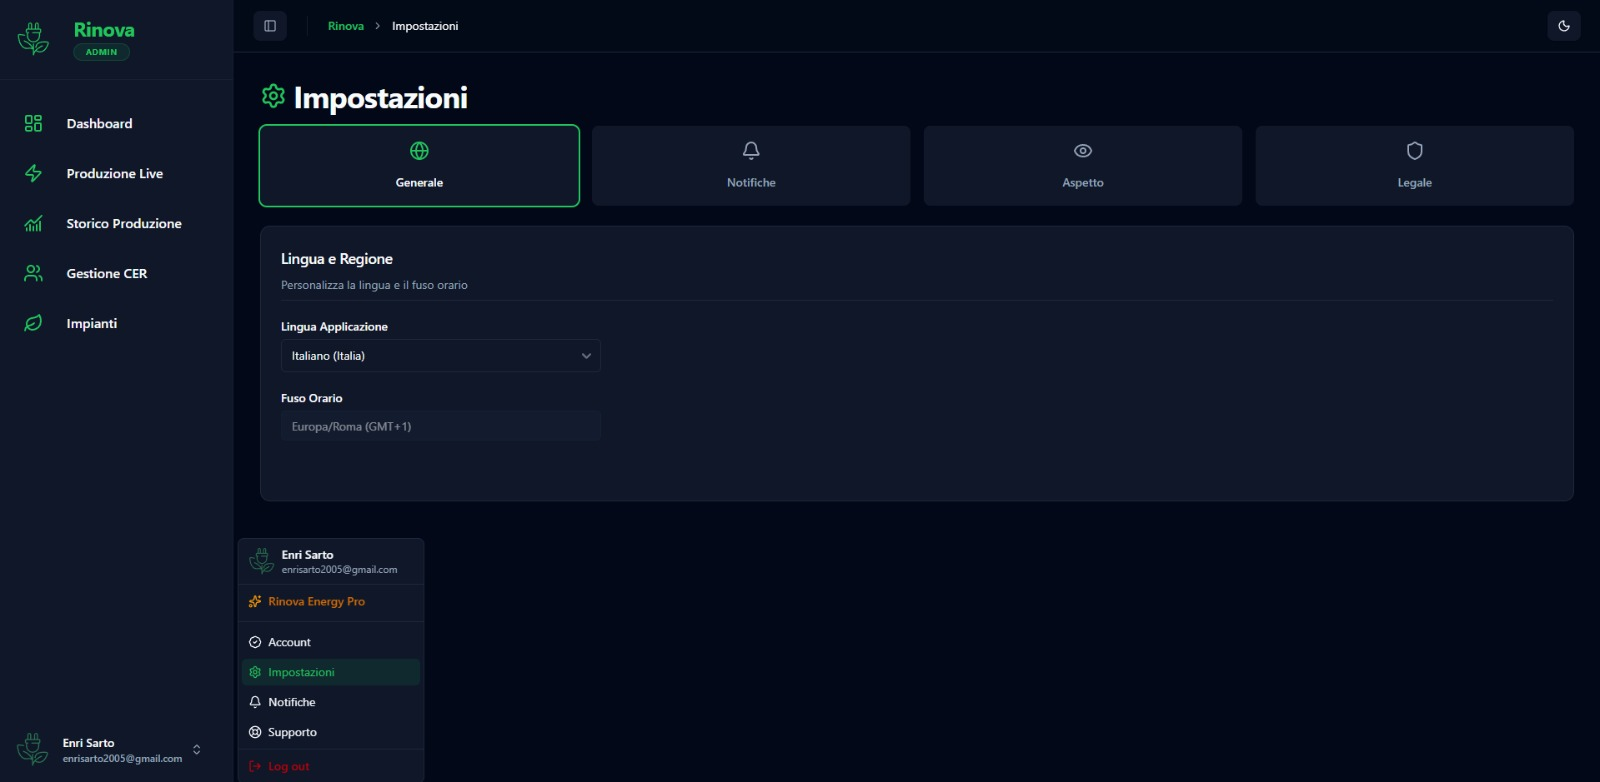
\includegraphics[width=1\textwidth]{images/frontend/schermata_areapersonalelogout.png}
    \caption{Menu utente e LogOut}
    \label{fig:areapersonalelogout}
\end{figure}

\begin{figure}[H]
    \centering
    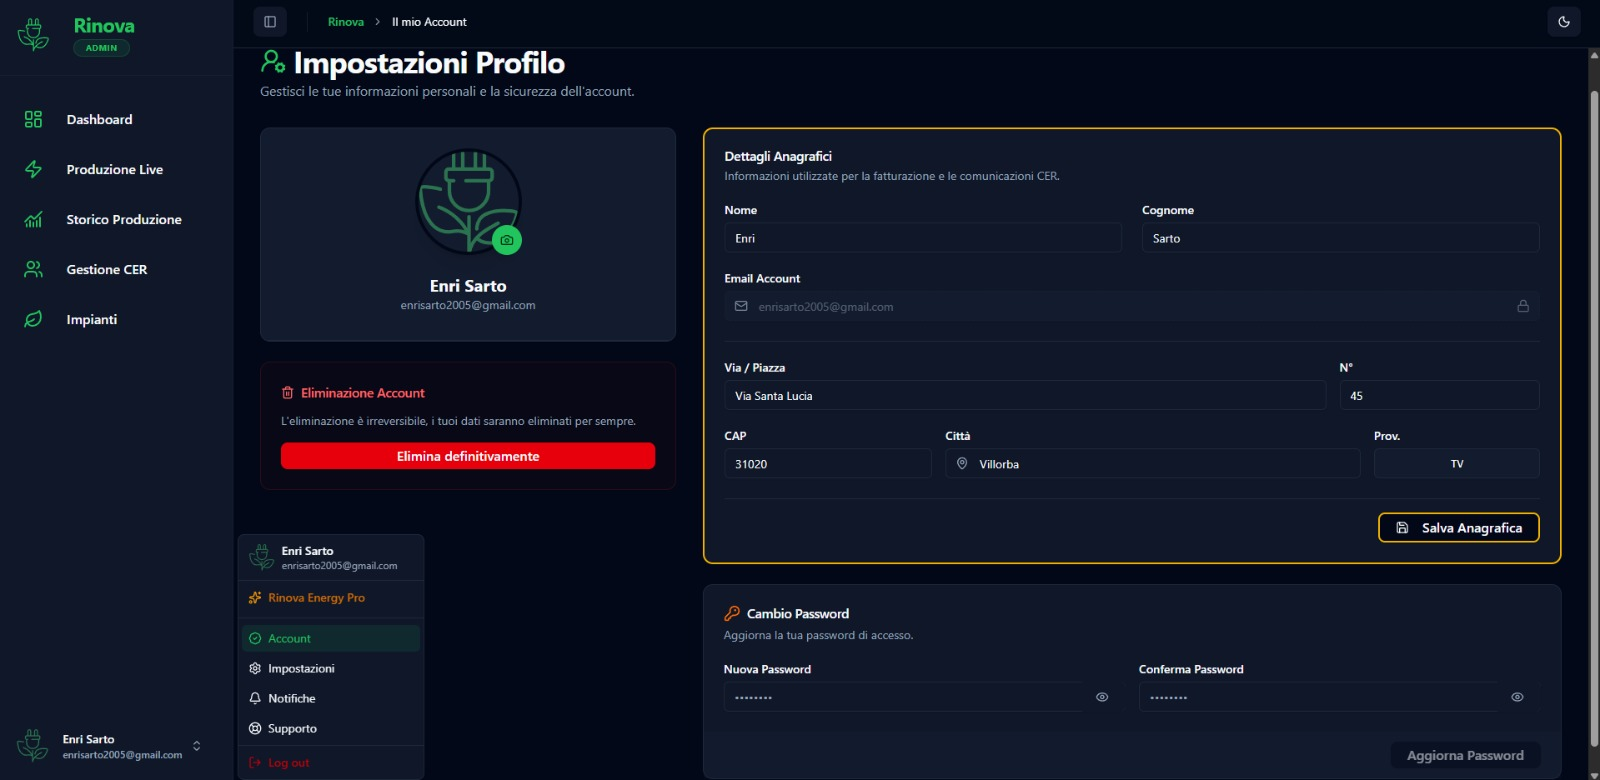
\includegraphics[width=1\textwidth]{images/frontend/schermata_impostazioni.png}
    \caption{Area personale}
    \label{fig:impostazioni}
\end{figure}

Le Figure \ref{fig:areapersonalelogout}  e \ref{fig:impostazioni} mostrano il Menu azioni utente e l'area personale.

\textbf{RF-03 e RF-03.1 - Area Personale:}
La sezione "Account" permette la modifica dei dati anagrafici e di accesso, confermando le modifiche solo dopo conferma esplicita attraverso i pulsanti "Salva anagrafica" e "Aggiorna password". Le tab ("Generale", "Notifiche", "Aspetto", "Legale") consentono una gestione granulare delle preferenze.

\textbf{RF-04 - Logout:}
Nel menu laterale (sidebar) in basso a sinistra, è chiaramente visibile e accessibile il comando "Log out" (evidenziato in rosso) per la terminazione sicura della sessione.

\textbf{RF-03.2 - Cancellazione:}
All'interno della tab "Account" è presente la funzionalità per l'eliminazione definitiva del profilo.

\textbf{RNF-06 - Privacy e GDPR:}
La sezione dedicata e la gestione granulare dei dati personali dimostrano la conformità alla normativa sulla privacy, garantendo all'utente il pieno controllo sulle informazioni memorizzate (Diritto all'oblio).

\subsubsection*{Supporto e Ticketing}
\begin{figure}[H]
    \centering
    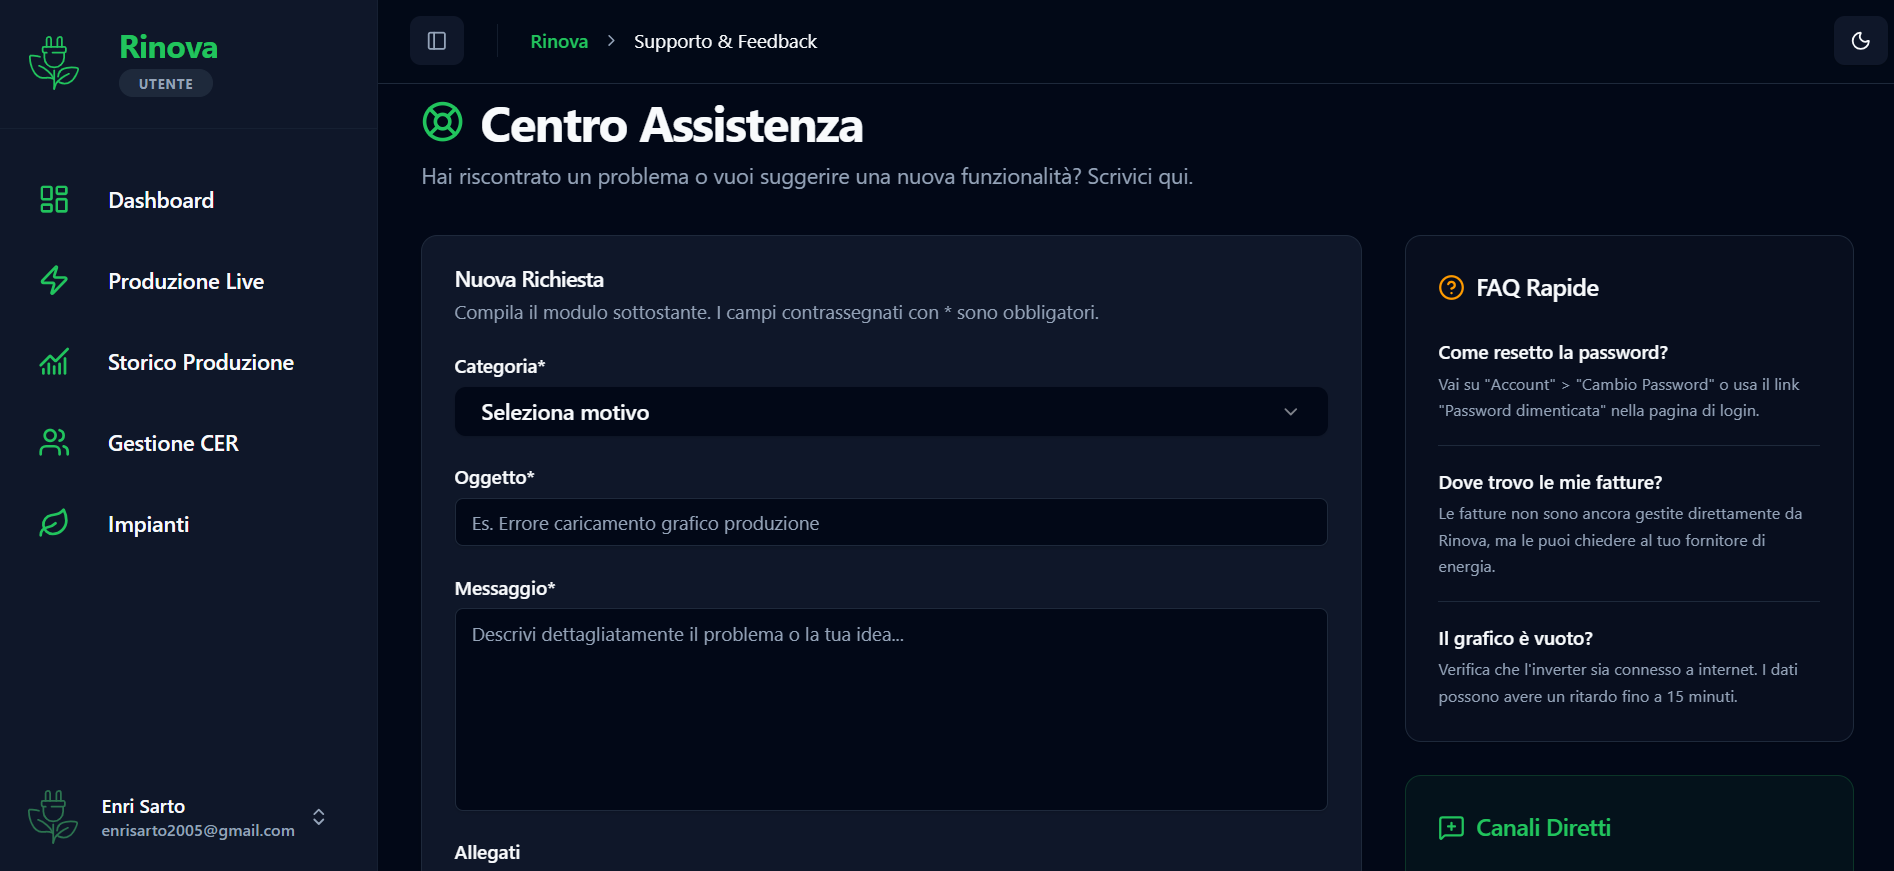
\includegraphics[width=1\textwidth]{images/frontend/schermata_ticket1.png}
    \caption{Centro Supporto e Feedback}
    \label{fig:supporto}
\end{figure}

\begin{figure}[H]
    \centering
    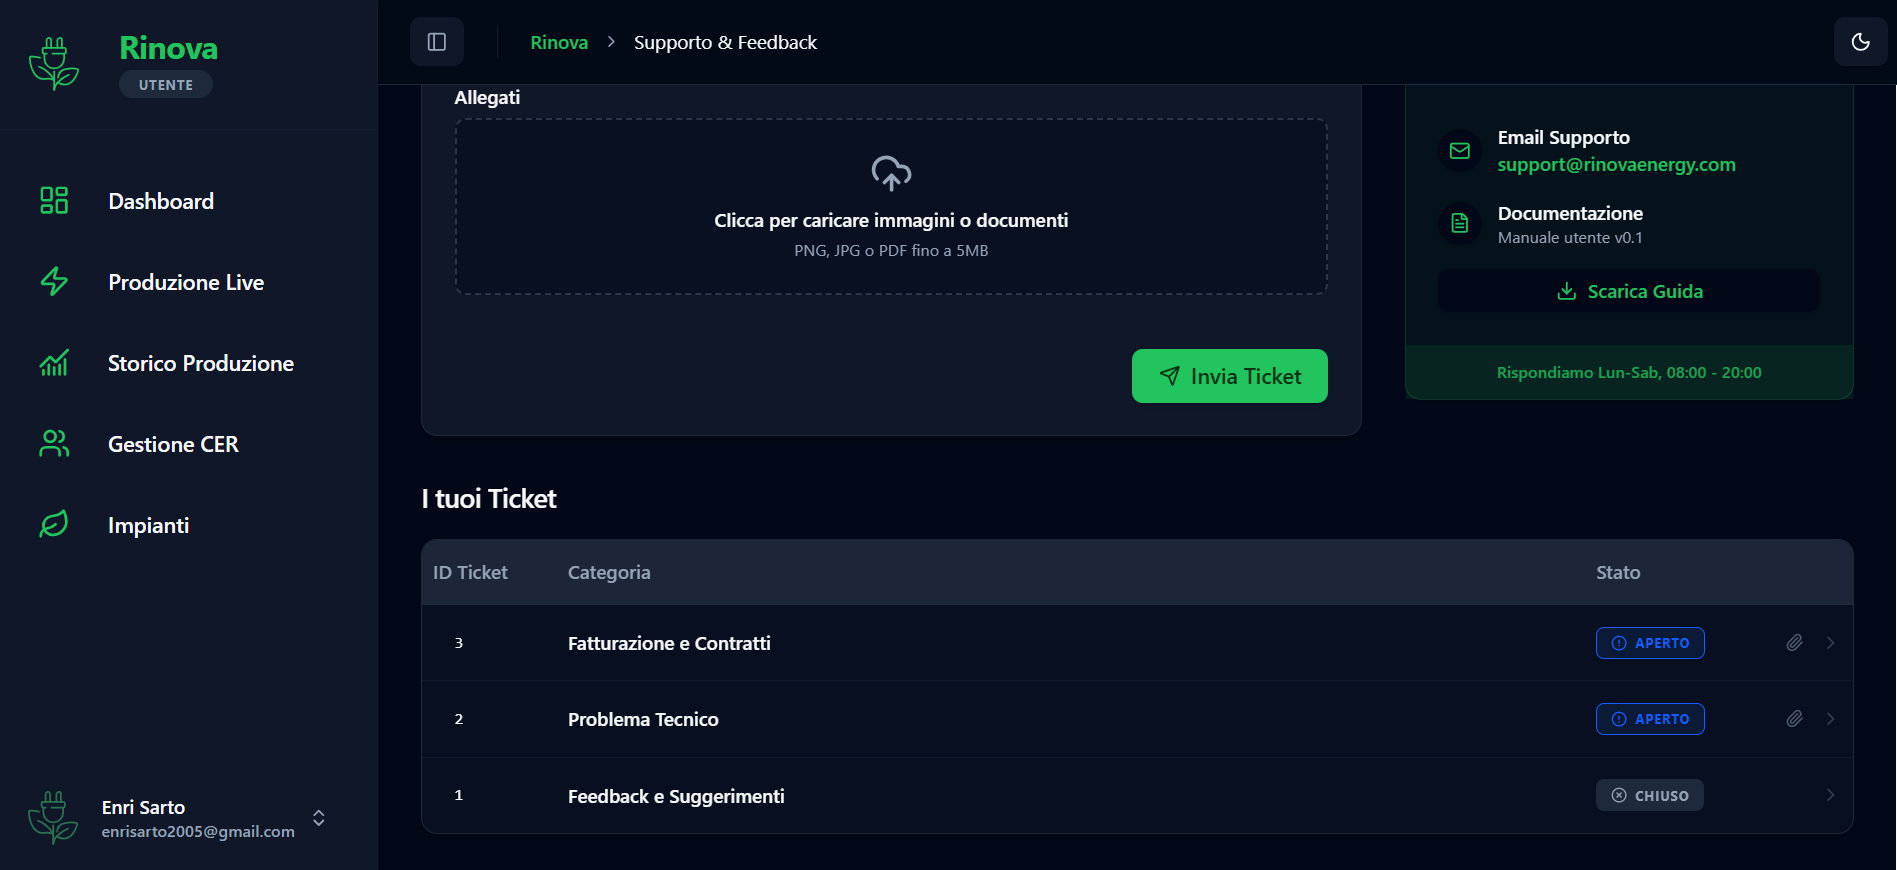
\includegraphics[width=1\textwidth]{images/frontend/schermata_ticket2.png}
    \caption{Dettaglio e Invio Ticket}
    \label{fig:supporto2}
\end{figure}

Le Figure \ref{fig:supporto} e \ref{fig:supporto2} illustrano il sistema di assistenza integrato.

\textbf{RF-10 - Apertura Ticket:}
L'interfaccia permette di aprire nuove segnalazioni tramite il pulsante "Invia Ticket" dopo aver riempito i campi del form. È presente un'area di drag-and-drop per allegare documenti o screenshot del problema.

\textbf{Persistenza e Stato:}
La tabella inferiore "I tuoi Ticket" mostra lo storico delle segnalazioni inviate, indicandone chiaramente lo stato (es. "APERTO", "CHIUSO") e la categoria (es. "Fatturazione", "Problema Tecnico"), garantendo la tracciabilità delle richieste.

\textbf{RNF-12 - Gestione Errori:}
Il sistema di upload (drag-and-drop) include controlli automatici sul formato e la dimensione dei file, prevenendo errori di caricamento e fornendo feedback immediati all'utente in caso di file non supportati.